  \subsection{Análisis de una señal modulada en frecuencia}

    Se procede a analizar una FM. Para ello se hace lo siguiente:

      \begin{figure}[H]
        \centering
          \frame{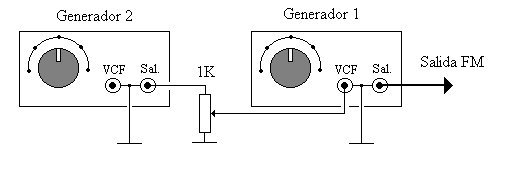
\includegraphics[width=0.8\textwidth]{Imagenes/ActividadPractica/6AnalisisDeUnaSeñalDeFM/EsquemaConexionGeneradores.png}}
          \caption{Conexión de los generadores.}
          \label{fig:FiguritaA}
      \end{figure}

    Inicialmente se procede a calibrar los generadores.

      \begin{figure}[H]
        \centering
        \begin{subfigure}[H]{0.48\textwidth}
          \frame{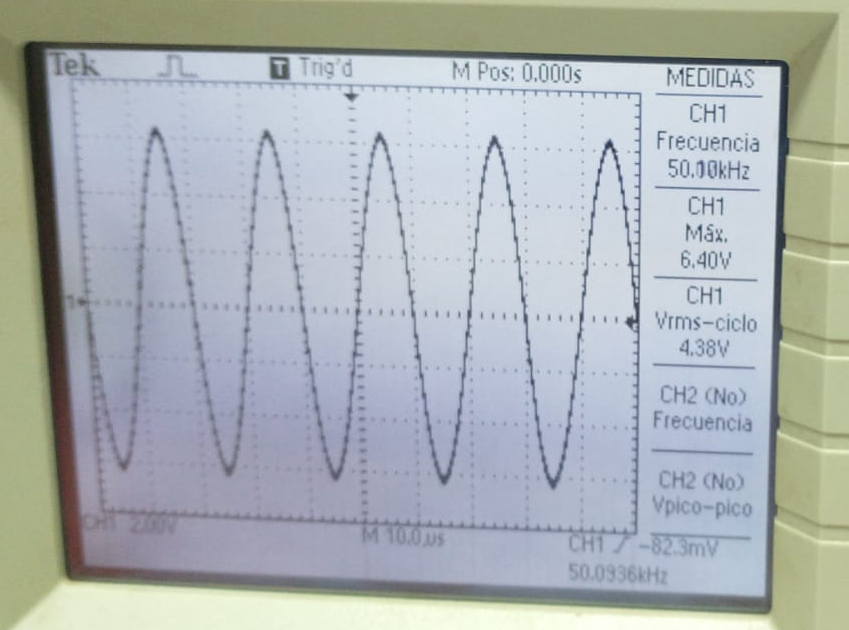
\includegraphics[width=\textwidth]{Imagenes/ActividadPractica/6AnalisisDeUnaSeñalDeFM/Exp6_Calibracion_G1.png}}
          \caption{Calibración G1.}
          \label{fig:FiguritaB}
        \end{subfigure}
        \hfill 
        \begin{subfigure}[H]{0.48\textwidth}
          \frame{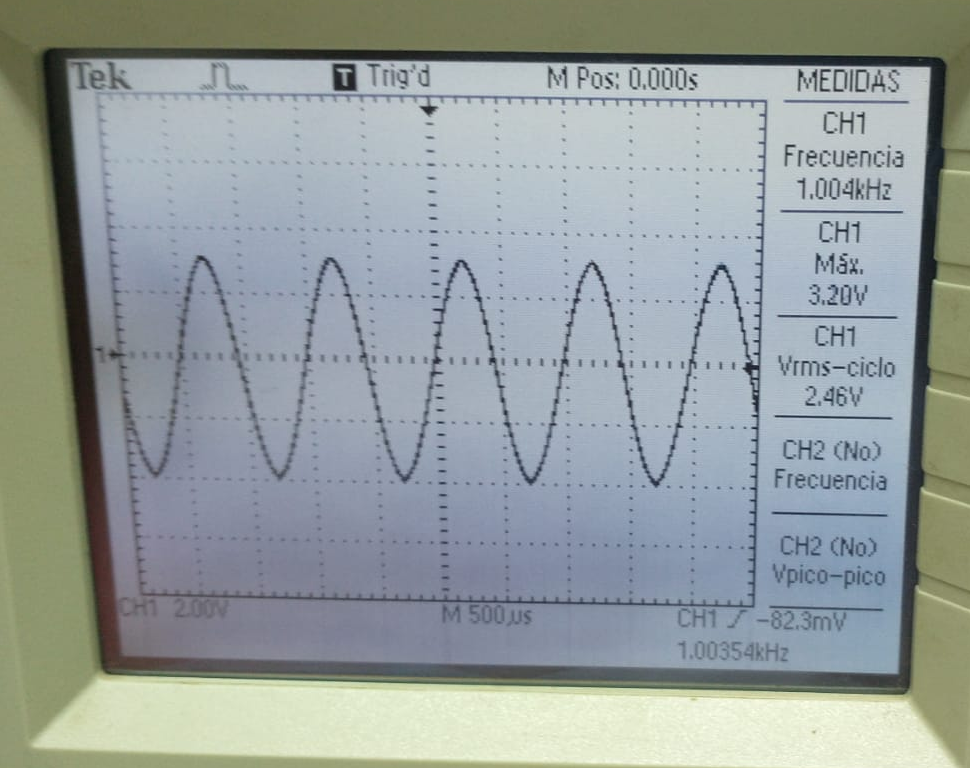
\includegraphics[width=\textwidth]{Imagenes/ActividadPractica/6AnalisisDeUnaSeñalDeFM/Exp6_Calibración_G2.png}}
          \caption{Calibración G2.}
          \label{fig:FiguritaC}
        \end{subfigure}
      \end{figure}

    Se observa la señal a 1 ms por div.

      \begin{figure}[H]
        \centering
          \frame{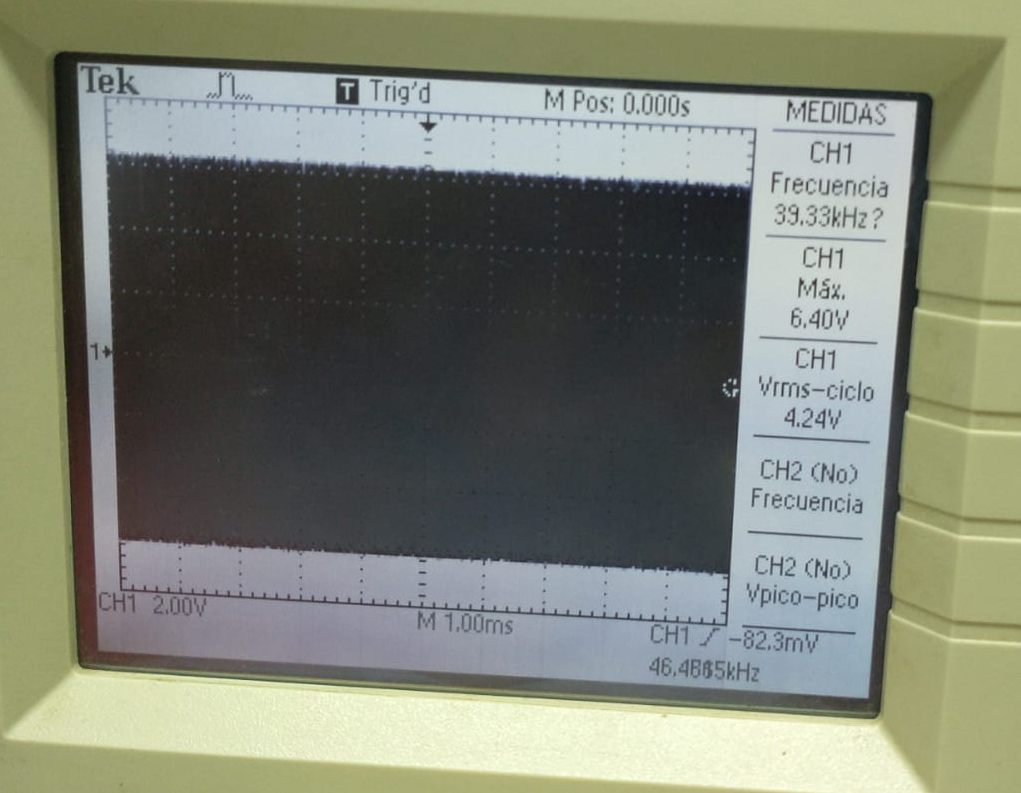
\includegraphics[width=0.8\textwidth]{Imagenes/ActividadPractica/6AnalisisDeUnaSeñalDeFM/Exp6_SeñalDeSalidaCon1msPorDiv.png}}
          \caption{Conexión de los generadores.}
          \label{fig:FiguritaA}
      \end{figure}

